%====================Step1====================%

%<*mtag101>
\begin{figure}[H]
\centering
\captionsetup{width=1\linewidth}
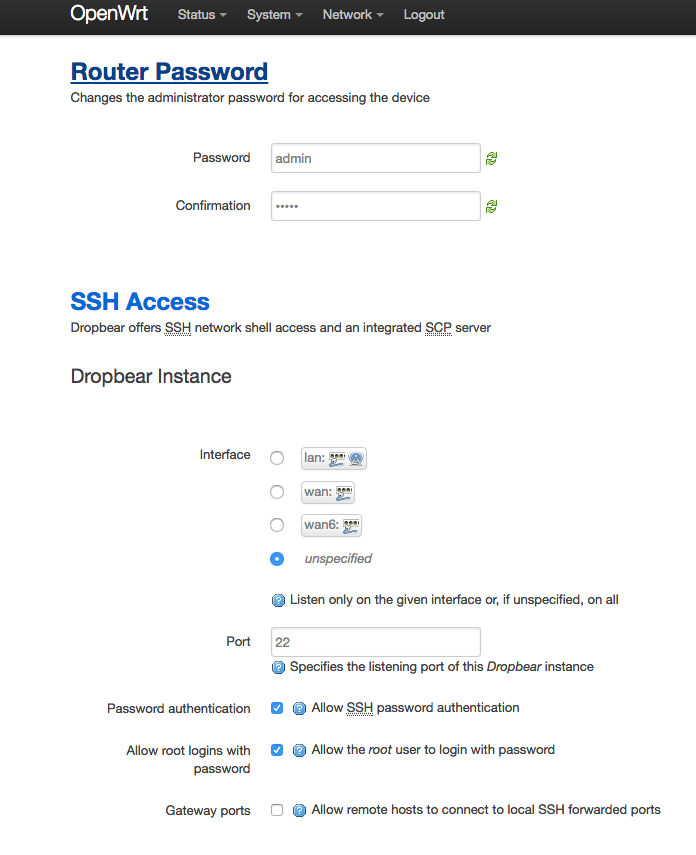
\includegraphics[scale=0.4]{\ImgPath/Ex3/Step1/ex3-1.png}
\caption{Configuring password / ssh }
\label{fig:1-1}
\centering
\end{figure}
%</mtag101>

%<*mtag102>
\begin{figure}[H]
\centering
\captionsetup{width=1\linewidth}
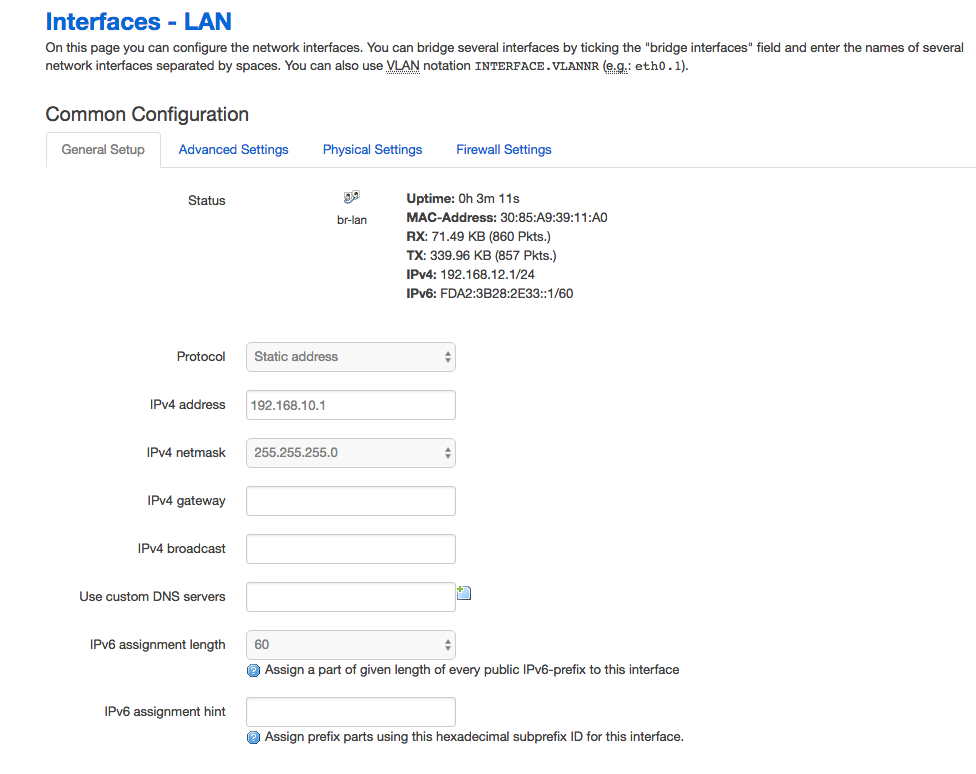
\includegraphics[scale=0.4]{\ImgPath/Ex3/Step1/ex3-2.png}
\caption{Configuring Static IP}
\label{fig:1-2}
\centering
\end{figure}
%</mtag102>

%<*mtag103>
\begin{figure}[H]
\centering
\captionsetup{width=1\linewidth}
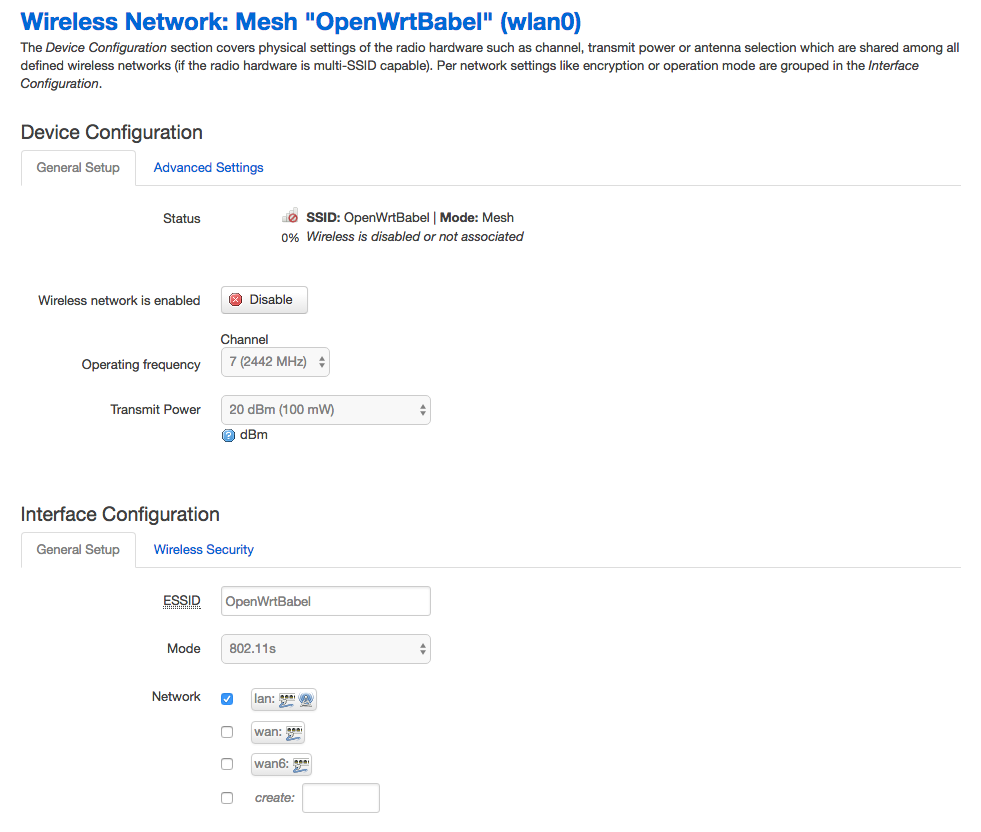
\includegraphics[scale=0.4]{\ImgPath/Ex3/Step1/ex3-3.png}
\caption{Configuring wireless mesh interface with 802.11s}
\label{fig:1-3}
\centering
\end{figure}
%</mtag103>

%<*mtag104>
\begin{figure}[H]
\centering
\captionsetup{width=1\linewidth}
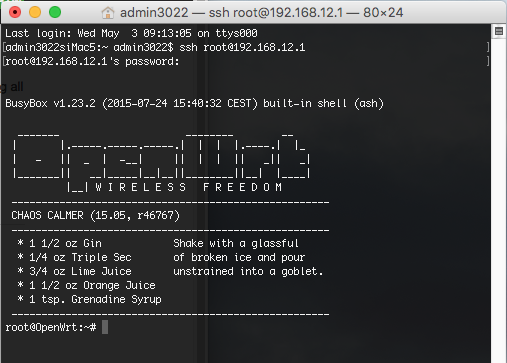
\includegraphics[scale=0.55]{\ImgPath/Ex3/Step1/ex3-4.png}
\caption{SSH proof to 192.168.11.1 OpenWrt Router}
\label{fig:1-4}
\centering
\end{figure}
%</mtag104>

%<*mtag105>
\begin{figure}[H]
\centering
\captionsetup{width=1\linewidth}
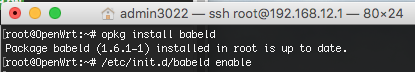
\includegraphics[scale=0.7]{\ImgPath/Ex3/Step1/ex3-5.png}
\caption{Installing and Enabling the Babel Daemon}
\label{fig:1-5}
\centering
\end{figure}
%</mtag105>

%<*mtag106>
\begin{figure}[H]
\centering
\captionsetup{width=1\linewidth}
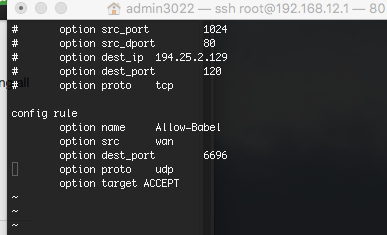
\includegraphics[scale=0.6]{\ImgPath/Ex3/Step1/ex3-6.png}
\caption{Editing the firewall configuration}
\label{fig:1-6}
\centering
\end{figure}
%</mtag106>

%<*mtag107>
\begin{figure}[H]
\centering
\captionsetup{width=1\linewidth}
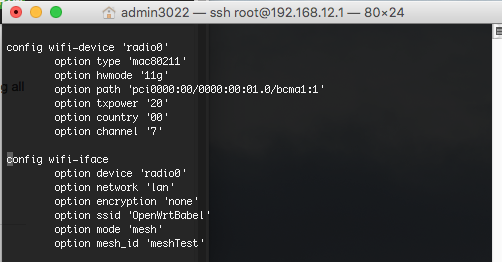
\includegraphics[scale=0.66]{\ImgPath/Ex3/Step1/ex3-7.png}
\caption{Editing the wireless configuration}
\label{fig:1-7}
\centering
\end{figure}
%</mtag107>

%<*mtag108>
\begin{figure}[H]
\centering
\captionsetup{width=1\linewidth}
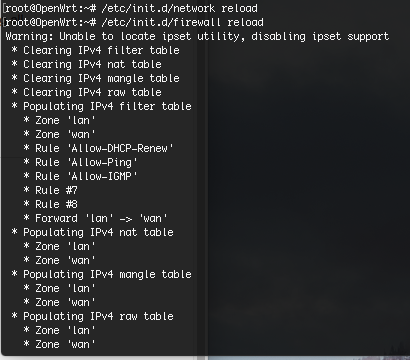
\includegraphics[scale=0.6]{\ImgPath/Ex3/Step1/ex3-8.png}
\caption{Reloading the firewall and network configurations}
\label{fig:1-8}
\centering
\end{figure}
%</mtag108>

%<*mtag109>
\begin{figure}[H]
\centering
\captionsetup{width=1\linewidth}
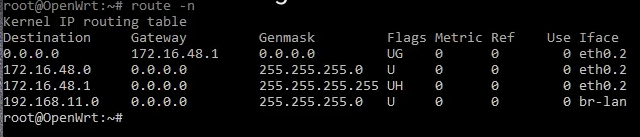
\includegraphics[scale=0.65]{\ImgPath/Ex3/Step1/ex3-9.png}
\caption{Checking the inital routing table}
\label{fig:1-9}
\centering
\end{figure}
%</mtag109>

%<*mtag110>
\begin{figure}[H]
\centering
\captionsetup{width=1\linewidth}
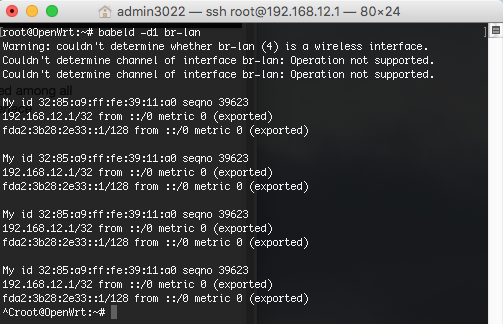
\includegraphics[scale=0.65]{\ImgPath/Ex3/Step1/ex3-10.png}
\caption{Preliminary test of the babel daemon}
\label{fig:1-10}
\centering
\end{figure}
%</mtag110>

%====================Step2====================%
%<*mtag201>
\begin{figure}[H]
\centering
\captionsetup{width=1\linewidth}
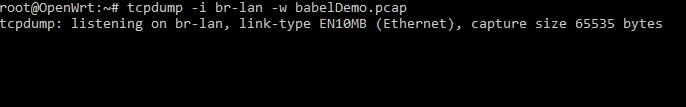
\includegraphics[scale=0.67]{\ImgPath/Ex3/Step2/3-11.png}
\caption{Starting inital packet capture}
\label{fig:2-1}
\centering
\end{figure}
%</mtag201>

%<*mtag202>
\begin{figure}[H]
\centering
\captionsetup{width=1\linewidth}
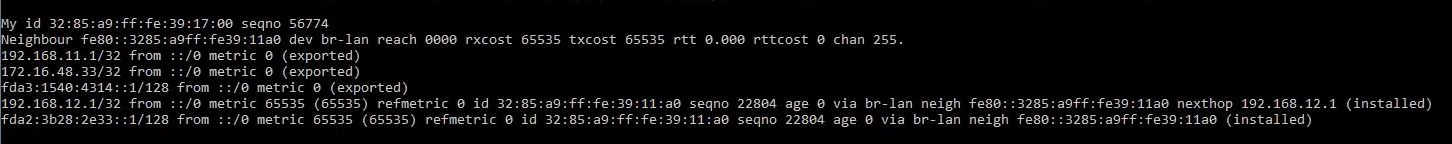
\includegraphics[scale=0.386]{\ImgPath/Ex3/Step2/3-12.png}
\caption{Proof of neighbor messages in the babel daemon debug}
\label{fig:2-2}
\centering
\end{figure}
%</mtag202>

%<*mtag203>
\begin{figure}[H]
\centering
\captionsetup{width=1\linewidth}
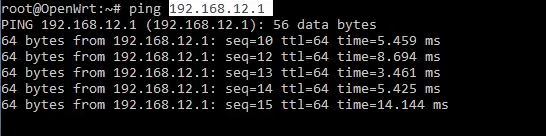
\includegraphics[scale=0.67]{\ImgPath/Ex3/Step2/3-13.png}
\caption{Proof of connectivity between 192.168.11.1 and 192.168.12.1 nodes}
\label{fig:2-3}
\centering
\end{figure}
%</mtag203>

%<*mtag204>
\begin{figure}[H]
\centering
\captionsetup{width=1\linewidth}
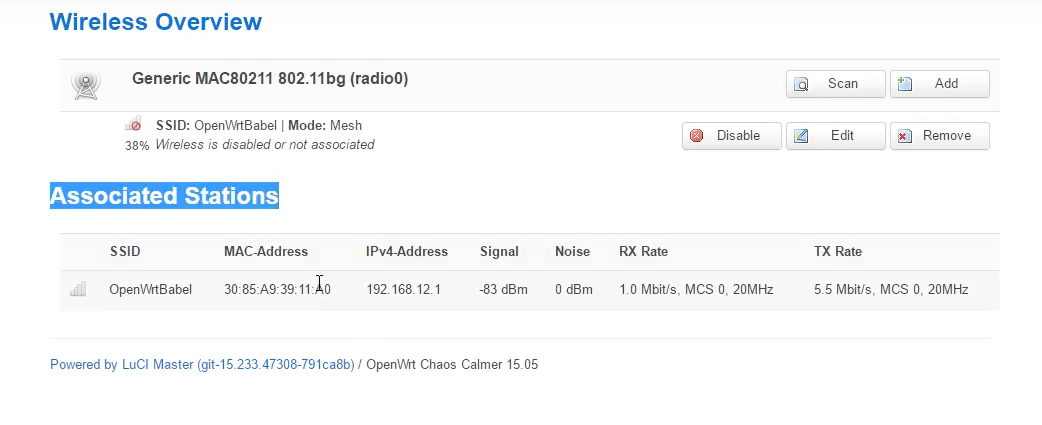
\includegraphics[scale=0.4]{\ImgPath/Ex3/Step2/3-14.png}
\caption{Verifying the Associated Stations in the OpenWrt GUI.}
\label{fig:2-4}
\centering
\end{figure}
%</mtag204>

%<*mtag205>
\begin{figure}[H]
\centering
\captionsetup{width=1\linewidth}
\includegraphics[scale=0.4]{\ImgPath/Ex3/Step2/3-15.png}
\caption{Checking the routing table first as Babel is running, and then after the babel daemon is stopped.}
\label{fig:2-5}
\centering
\end{figure}
%</mtag205>

%<*mtag206>
\begin{figure}[H]
\centering
\captionsetup{width=1\linewidth}
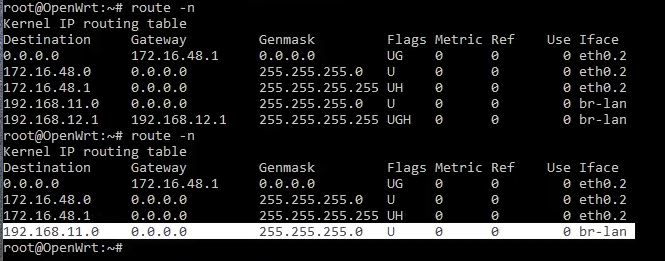
\includegraphics[scale=0.67]{\ImgPath/Ex3/Step2/3-16.png}
\caption{Checking the routing table first as Babel is running, and then after the babel daemon is stopped.}
\label{fig:2-6}
\centering
\end{figure}
%</mtag206>

%<*mtag207>
\begin{figure}[H]
\centering
\captionsetup{width=1\linewidth}
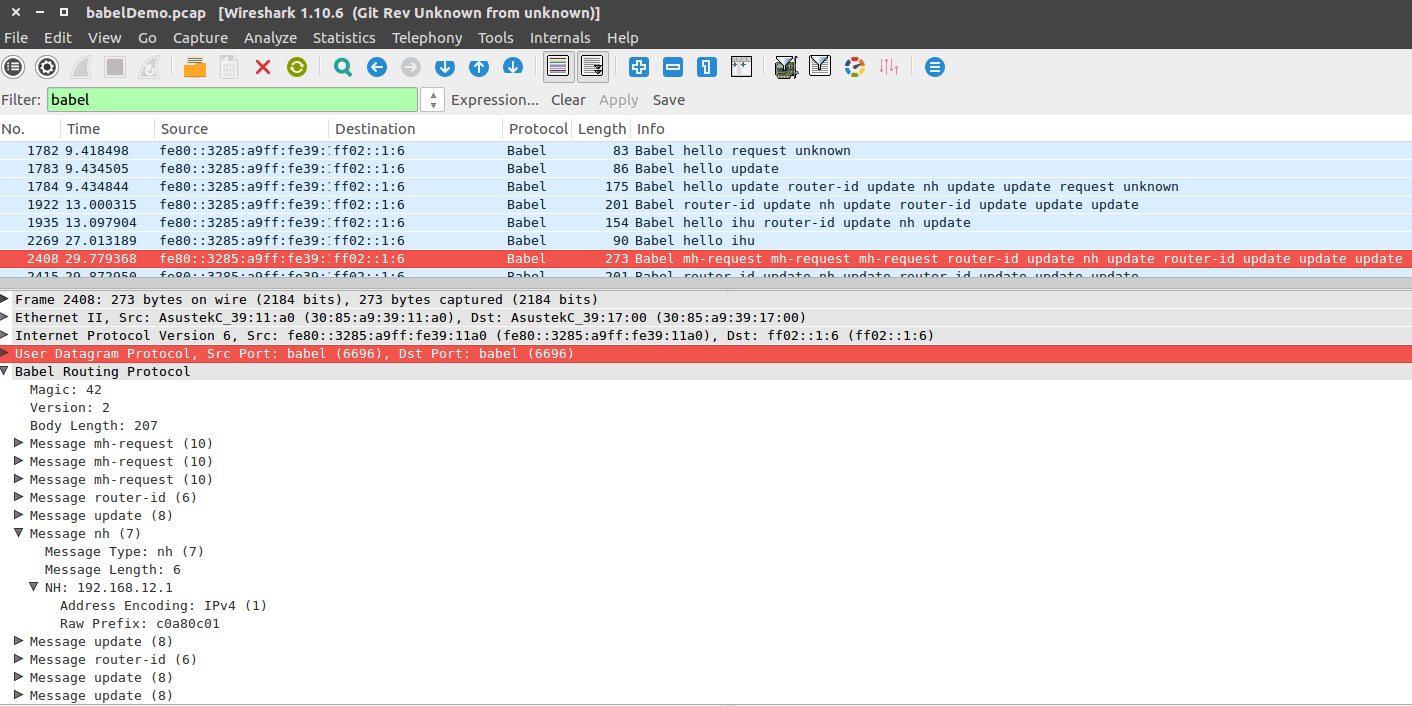
\includegraphics[scale=0.35]{\ImgPath/Ex3/Step2/3-17.png}
\caption{Example of finalized wireshark capture}
\label{fig:2-7}
\centering
\end{figure}
%</mtag207>
%====================Step3====================%
%<*mtag300>
\begin{figure}[H]
\centering
\captionsetup{width=1\linewidth}
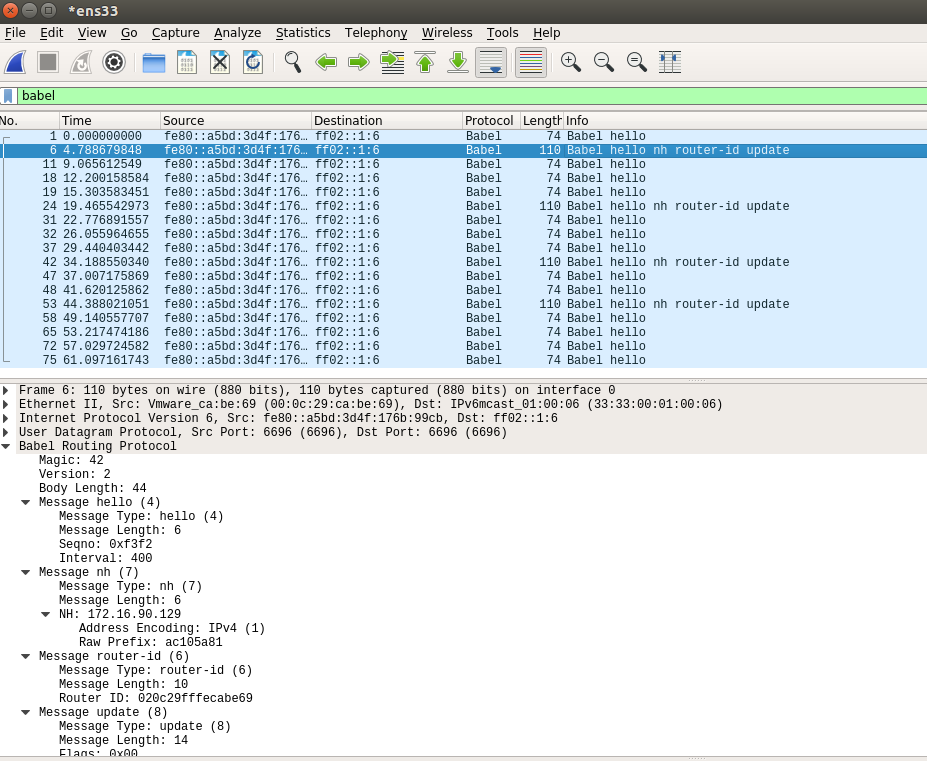
\includegraphics[scale=0.4]{\ImgPath/Ex3/Step3/Selection_001.png}
\caption{}
\label{fig:Ex2S3_1}
\centering
\end{figure}
%</mtag300>